\documentclass[a4paper,11pt]{article}
\setlength{\parindent}{0pt}

\usepackage[ruled,vlined]{algorithm2e}
\usepackage{mlsubmit}
\usepackage{graphicx}
\usepackage{subfig}

\begin{document}

\graphicspath{ {./P6/Plots/} }

\initmlsubmision{2} % assignment number
{Utkarsh Gupta}   % your name
{180836}	% your roll number

\begin{mlsolution}

The Logistic Regression loss function is given by:

\begin{equation*}
    L(\vw) = -\sum_{n=1}^{N}(y_n\vw^T\vx_n - \text{log}(1+\text{exp}(\vw^T\vx_n)))
\end{equation*}
\begin{equation*}
    \implies L(\vw) = -\sum_{n=1}^{N}(y_n\text{log}(\sigma(\vw^T\vx_n)) + (1-y_n)\text{log}(1-\sigma(\vw^T\vx_n)))
\end{equation*}

Taking derivative with respect to $\vw$ we get the gradient $\vg^{(t)}$ as:

\begin{equation*}
    \vg^{(t)} = \sum_{n=1}^{N}(-y_n\vx_n(1-\sigma(\vw^T\vx_n))+(1-y_n)\vx_n\sigma(\vw^T\vx_n))=\sum_{n=1}^{N}(\vx_n(\sigma(\vw^T\vx_n)-y_n)) = \vX^T(\hat{\vy}-\vy)
\end{equation*}

Hessian is nothing but the second derivative of $\vg^{(t)}$:

\begin{equation*}
    \vH^{(t)}=\vec{\nabla}^2L(\vw)=\sum\limits_{n=1}^{N}(\frac{\partial \vg^{(t)}}{\partial \vw^T})=\sum\limits_{n=1}^{N}(\vx_n\vx_n^T\sigma(\vw^T\vx_n)(1-\sigma(\vw^T\vx_n)))
\end{equation*}

This is equivalent to concatenating column vectors $\vx_v\in\mathbb{R}^D$ into a matrix $X$ of size $D\times N$ such that $\sum_{n=1}^N \vx_n\vx_n^T=\vX\vX^T$. The scalar terms are combined in a diagonal matrix $\vR$ such that $R_{ii}=\sigma(\vw^T\vx_i)(1-\sigma(\vw^T\vx_i))$.

\begin{equation*}
    \vH^{(t)} = \vX\vR^{(t)}\vX^T
\end{equation*}

Substituting the Hessian and Gradient in the weight update equation we get, (so far we wrote $\vw^{(t)}$ as $\vw$):

\begin{equation*}
    \vw^{(t+1)} = \vw^{(t)} - (\vX\vR^{(t)}\vX^T)^{-1}\vX^T(\hat{\vy}-\vy)
\end{equation*}

\begin{equation} \label{eq:1}
    \implies \vw^{(t+1)} = (\vX\vR^{(t)}\vX^T)^{-1}\vX^T\vR^{(t)}(\vX\vw^{(t)} - \vR^{-1}(\hat{\vy}-\vy))
\end{equation}

The solution obtained looks suspiciously familiar. The given weighted least squares problem can be written as ($\vC^{(t)}$ is a diagonal matrix with $C_{nn} = \gamma_n^{(t)}$):

\begin{equation*}
    \vw^{(t+1)} = \text{arg}\min\limits_\vw\sum_{n=1}^N\gamma_n^{(t)}(\hat{y}^{(t)}-\vw^T\vx_n)^2 = \text{arg}\min\limits_\vw (\hat{\vY}^{(t)}-\vX\vw)^T\vC^{(t)}(\hat{\vY}^{(t)}-\vX\vw)
\end{equation*}

Taking the derivative and setting it to $0$, we get:

\begin{equation} \label{eq:2}
    \vw^{(t+1)} = (\vX^T\vC^{(t)}\vX)^{-1}\vX^T\vC^{(t)}\hat{\vY}^{(t)}
\end{equation}

Comparing \ref{eq:2} with \ref{eq:1}, we get:

\[
    \boxed{
        \vC^{(t)} = \vR^{(t)}\\
        \implies \gamma_n^{(t)} = \sigma(\vw^{(t)T}\vx_n)(1-\sigma(\vw^{(t)T}\vx_n))
    }
\]\\
\[
    \boxed{
        \hat{\vY}^{(t)} = (\vX\vw^{(t)} - \vR^{-1}(\hat{\vy}-\vy))
        \implies \hat{y}^{(t)}_n = \vw^{(t)T}\vx_n - \frac{\sigma(\vw^{(t)T}\vx_n) - y_n}{\sigma(\vw^{(t)T}\vx_n)(1-\sigma(\vw^{(t)T}\vx_n))}
    }
\]\\

We know that in case of Logistic Regression $\sigma(\vw^{(t)T}\vx_n)$ represents the probability that an input $\vx_n$ belongs to the "0" class.
If we let $\sigma(\vw^{(t)T}\vx_n) = p_n$ then $\gamma_n^{(t)} = p_n(1-p_n)$, which attains it's maximum value at $p_n = \frac{1}{2}$, this implies that the loss function gives more weightage to those examples that lie close to the decision boundary. Thus, the expression intuitively makes sense.

\end{mlsolution}

\begin{mlsolution}

We know that the weights obtained from perceptron algorithm can be written as;

\begin{equation*}
    \vw = \sum_{i=1}^N\alpha_iy_i\vx_i
\end{equation*}

where $\alpha_i$ is the number of times $\vx_i$ was missclassified, and hence, caused $\vw$ to update. Substituting this result in the original perceptron algorithm we get:

\begin{equation*}
    \begin{split}
        \hat{y}{}& = sgn(\vw^T\vx) = sgn((\sum_{i=1}^N\alpha_iy_i\vx_i)^T\vx)\\
        & = sgn(\sum_{i=1}^N\alpha_iy_i(\vx_i\cdot\vx))
    \end{split}
\end{equation*}

Since we have an inner product, we can apply the Kernel trick. The inner product can now be replaced directly thereby, taking benefit of the Feature Map $\phi$ without explicitly calculating it.

\begin{equation*}
    \hat{y} = sgn(\sum_{i=1}^N\alpha_iy_i\vK(\vx_i,\vx))
\end{equation*}

The algorithm below gives the required initialization, mistake condition and update equation. $K$ is the number of iterations for which we want the algorithm to run. $\vX$ and $\vY$ correspond to the input features and outputs respectively. \\

\begin{algorithm}[H]
\DontPrintSemicolon
\SetAlgoLined
\SetKwFunction{KPerceptron}{K\_Perceptron}
\SetKwFunction{FSub}{sub\_grad}
\SetKwProg{Fn}{Function}{:}{\KwRet}
\Fn{\KPerceptron{$\vX, \vY, K$}}{
    \tcp{Initialization}
    $\pmb{\alpha} :=$ zero $N$ x 1 vector\\
    \For{$k=1$ to $K$}{
        \For{$j=1$ to $N$}{
            $\hat{y} = sgn(\sum_{i=1}^N\alpha_iy_i\vK(\vx_i,\vx_j))$\\
            \tcp{Mistake Condition}
            \uIf{$\hat{y}\neq y_j$}{
                \tcp{Update equation}
                $\alpha_j = \alpha_j + 1$
            }
        }
    }
}
\Repeat{convergence}{
    \KPerceptron{$\vX, \vY, K$}
}
\caption{Kernel Perceptron}
\end{algorithm}


\end{mlsolution}

\begin{mlsolution}

The primal formulation of the Imbalanced Class SVM is:
\begin{equation*}
    \min\limits_{\vw, b, \pmb{\xi}} \frac{||\vw||^2}{2}+\sum\limits_{n=1}^NC_{y_n}\xi_n
\end{equation*}
subjected to $y_n(\vw^T\vx_n+b)\geq1-\xi_n$ and $\xi_n\geq0 \; \forall n$.

The Langrangian is given by:
\begin{equation*}
    \min\limits_{\vw, b, \pmb{\xi}} \; \max\limits_{\pmb{\alpha}\geq\pmb{0}, \pmb{\beta}\geq\pmb{0}} \cL(\vw, \; b, \pmb{\xi}, \pmb{\alpha}, \pmb{\beta}) = \frac{||\vw||^2}{2}+\sum\limits_{n=1}^NC_{y_n}\xi_n + \sum\limits_{n=1}^N\alpha_n\bc{1-y_n(\vw^T\vx_n+b)-\xi_n} - \sum\limits_{n=1}^N\beta_n\xi_n
\end{equation*}

Taking partial derivatives of $\cL$ w.r.t. $\vw$, $b$ and $\xi_n$ and setting to zero gives:

\[
    \frac{\partial \cL}{\partial \vw}=0 \implies \boxed{\vw = \sum\limits_{n=1}^N\alpha_ny_n\vx_n}\; ,\; \frac{\partial \cL}{\partial b}=0 \implies \boxed{\sum\limits_{n=1}^N\alpha_ny_n = 0}\; ,\; \frac{\partial \cL}{\partial \xi_n}=0 \implies \boxed{C_{y_n}-\alpha_n-\beta_n=0}
\]

Using $\beta_n\geq0$ and $C_{y_n}-\alpha_n-\beta_n=0$, we get: $0\leq\alpha_n\leq C_{y_n}$.

Substituting these in the original $\cL$, we get the Dual Langrangian:

\[
    \boxed{\max\limits_{\pmb{\alpha}\leq\vC, \pmb{\beta}\geq\pmb{0}} \cL_D(\pmb{\alpha}, \pmb{\beta}) = \sum\limits_{n=1}^N\alpha_n - \frac{1}{2}\sum\limits_{m,n=1}^N\alpha_m\alpha_ny_my_n(\vx_m^T\vx_n) \;\;\; s.t. \;\; \sum\limits_{n=1}^N\alpha_ny_n=0}
\]
\[
    \boxed{\max\limits_{\pmb{\alpha}\leq\vC} \cL_D(\pmb{\alpha}) = \pmb{\alpha}^T\pmb{1} - \frac{1}{2}\pmb{\alpha}^T\pmb{G\alpha} \;\;\; s.t. \;\; \sum\limits_{n=1}^N\alpha_ny_n=0}
\]
$\vC$ is a $N$x1 vector with $n^{th}$ entry being $C_{y_n}$. As observed earlier in case of soft-margin SVM, the dual variables $\pmb{\beta}$ do not affect the Dual Problem. The $\pmb{\alpha}$ vector will be sparse as well (KKT conditions) and non-zero $\alpha_n$ will correspond to the support vectors. \\ \\
In the standard SVM, $\vC$ is a vector having all values as $C$ (a fixed scalar). This performs well for balanced classes but as the data becomes imbalanced, the ratio between the positive and negative support vectors also becomes imbalanced.\\ \\
This causes the separating hyperplane to be skewed towards the minority class, which finally yields a suboptimal model. In the new problem setting, the misclassification cost vector $\vC$ is redefined. By assigning a higher misclassification cost for the minority class examples than the majority class examples, the aforementioned effect of class imbalance can be reduced.
Let's assume that negative examples are in minority, then if we make $C_{\textbf{-1}} > C_{\textbf{+1}}$, we assign a higher cost of misclassification to negative class example. Thus, we can achieve the desired effect.

\end{mlsolution}

\begin{mlsolution}

In order to perform step 1, we can calculate distances from all the cluster means and then assign the incoming point $\vx_n$ to the cluster whose cluster mean has the least distance from the incoming point. In other words, we can solve the following optimization problem:

\begin{equation*}
    \hat{k} = \text{arg} \min\limits_k ||\pmb{\mu_k} - \vx_n||
\end{equation*}

After we perform Step 1 in an online setting, the gradient required for update will be with respect to $\vx_n$ only:

\begin{equation*}
    \frac{\partial \cL}{\partial \pmb{\mu_{\hat{k}}}} = -2(\vx_n - \pmb{\mu_{\hat{k}}})
\end{equation*}

Thus, update equation we use will be:

\begin{equation*}
    \pmb{\mu_{\hat{k}}} = (1-\eta)\pmb{\mu_{\hat{k}}} + \eta\vx_n
\end{equation*}

where $\eta$ is the learning rate. A good choice for it could be $\frac{1}{\cV[\hat{k}]}$, i.e., the inverse of the new total number of points in the cluster $\hat{k}$. The SGD based K-means algorithm can be summarised as:\\

\begin{algorithm}[H]
    \DontPrintSemicolon
    \SetAlgoLined
    \SetKwFunction{SGDKmeans}{SGD\_K\_Means}
    \SetKwFunction{InitX}{Initialize}
    \SetKwProg{Fn}{Function}{:}{\KwRet}
    \Fn{\SGDKmeans{$\vx_n, K, \bs{\pmb{\mu_1, \mu_2, \dots, \mu_K}}$}}{
        $\hat{k} = -1$\\
        $d = \textsc{infinity}$\\
        \tcp{Find the cluster nearest to the input point}
        \For{$k=1$ to $K$}{
            \uIf{$||\pmb{\mu_k}-\vx_n||\leq d$}{
                $d = ||\pmb{\mu_k}-\vx_n||$\\
                $\hat{k} = k$\\
            }
        }
        $\cV[\hat{k}] = \cV[\hat{k}]+1$ \tcp*{Increase the count of points in the cluster}
        $\eta = 1/\cV[\hat{k}]$ \tcp*{Set learning rate}
        $\pmb{\mu_{\hat{k}}} = (1-\eta)\pmb{\mu_{\hat{k}}} + \eta \vx_n$ \tcp*{The cluster-mean update equation}
    }
    \Fn{\InitX{$\vX, K$}}{
        $\mathbf{\cV} :=$ zero $K$ x 1 vector \tcp*{Set the number of inputs in each cluster.}
        $\pmb{\mu_i} :$ Randomly Initialize Cluster means.\\
        \Repeat{convergence}{
            \For{each $\vx_i$ in $\vX$}{
                \SGDKmeans($\vx_n, K, \bs{\pmb{\mu_1, \mu_2, \dots, \mu_K}}$)
            }
        }
    }
    \caption{SGD based Online K-Means Clustering}
\end{algorithm}

\pagebreak

The update equation makes sense as it gives weightage to both the existing means and the new point. Initially, when the means are set randomly, learning rate $\eta$ is high ($=1$) which makes sense as the assigned point is a better choice over the randomly selected mean. 
As the algorithm progresses, we encounter more points, and the learning rate falls. The update equation takes into account the fact that the present cluster mean represents the points in the cluster encountered so far and hence, assigns it a weight in proportion to it ($1-\eta$). 
The term $\eta \vx_n$ takes in the information from the new point added to the cluster and incorporates it into the new cluster mean. All this ensures that contribution from each element is the same (as it would be in true cluster mean). Thus, we can see how both the update equation and the learning rate make sense.


\end{mlsolution}
	
\begin{mlsolution}

The two major steps of K-means are Cluster assignment and Cluster mean update. For Kernel K-means with feature map $\phi$ we have:

\begin{equation*}
    z_n = \text{arg}\min\limits_k ||\phi(\vx_n) - \phi(\pmb{\mu_k})||^2 \;\;\; \dots \text{Cluster Assignment}
\end{equation*}

\begin{equation*}
    \phi(\pmb{\mu_k}) = \frac{1}{N_k} \sum\limits_{\vx_n | z_n=k}\phi(\vx_n) \;\;\;\;\;\;\;\;\;\;\;\;\;\; \dots \text{Cluster Mean Update}
\end{equation*}

We can convert the cluster assignment to inner product form in order to apply the kernel trick:

\begin{equation*}      
    ||\phi(\vx_n) - \phi(\pmb{\mu_k})||^2= \phi(\vx_n)^T\phi(\vx_n) - 2\phi(\vx_n)^T\phi(\pmb{\mu_k}) + \phi(\pmb{\mu_k})^T\phi(\pmb{\mu_k})
\end{equation*}
\begin{equation*}
    \implies||\phi(\vx_n) - \phi(\pmb{\mu_k})||^2=\cK(\vx_n, \vx_n) -2\cK(\vx_n, \pmb{\mu_k}) + \cK(\pmb{\mu_k},\pmb{\mu_k})
\end{equation*}

An important thing to note here is the fact how $\pmb{\mu_k}$ are (can be) calculated:

\begin{equation*}
    \pmb{\mu_k} = \phi^{-1} (\frac{1}{N_k} \sum\limits_{\vx_n | z_n=k}\phi(\vx_n))
\end{equation*}

Clearly, if we have an infinite dimensional feature space, we won't be able to store the actual cluster mean but can perform step 1 using the Kernel Trick, as discussed earlier.
We can get around the apparent problem by not explicitly calculating the cluster means. We can assign random values to $\pmb{\mu_k}$ to obtain initial values of $z_n$.
We can then continue to re-assign clusters by combining the two steps. Substituting $\phi(\pmb{\mu_k})$ in the kernelised assignment equation we get:

\begin{equation*}
    z_n = \text{arg}\min\limits_k \bc{\phi(\vx_n)^T\phi(\vx_n) - \frac{2}{N_k}\phi(\vx_n)^T\sum\limits_{\vx_i | z_i=k}\phi(\vx_i) + \frac{1}{N_k^2}\sum\limits_{\vx_i, \vx_j | z_i=z_j=k}\phi(\vx_i)^T\phi(\vx_j)}
\end{equation*}

\begin{equation*}
    \implies z_n = \text{arg}\min\limits_k \bc{\cK(\vx_n,\vx_n) - \frac{2}{N_k}\sum\limits_{\vx_i | z_i=k} \cK(\vx_n, \vx_i) + \frac{1}{N_k^2}\sum\limits_{\vx_i, \vx_j | z_i=z_j=k}\cK(\vx_i, \vx_i)}
\end{equation*}

\pagebreak
The entire process can be summarised in the following algorithm:
\begin{algorithm}
    \DontPrintSemicolon
    \SetAlgoLined
    \For{$k = 1\; to\; K$}{
        $N_k:=$0
    }
    $\pmb{\mu_i} :$ Randomly Initialize cluster means.\tcp*{Initialization}
    \For{$n=1\; to\; N$}{
        $\hat{k} = \text{arg}\min_k \cK(\vx_n, \vx_n) -2\cK(\vx_n, \pmb{\mu_k}) + \cK(\pmb{\mu_k},\pmb{\mu_k})$\\
        $z_n=\hat{k}$ \tcp*{Initial Cluster Assignment}
        $N_{\hat{k}}=N_{\hat{k}}+1$
    }
    \Repeat{convergence}{
        \For{$n=1\; to\; N$}{
            $k' = z_n$\\
            $\hat{k} = \text{arg}\min\limits_k \bc{\cK(\vx_n,\vx_n) - \frac{2}{N_{k'}}\sum\limits_{\vx_i | z_i=k'} \cK(\vx_n, \vx_i) + \frac{1}{N_{k'}^2}\sum\limits_{\vx_i, \vx_j | z_i=z_j=k'}\cK(\vx_i, \vx_i)}$\\
            $z_n=\hat{k}$ \tcp*{Cluster Re-assignment (Update)}
            $N_{k'}=N_{k'}-1$\\
            $N_{\hat{k}}=N_{\hat{k}}+1$\\
        }
    }
    \caption{Kernel K-Means}
\end{algorithm}

An interesting thing to note here is that similar to classic K-means, we have the Initialization and Updation phase but unlike classic K-means, we do not have the explicit Mean Computation step. The means are never explicitly calculated and the updates are made using the Kernel trick and number of cluster points directly. \\

In case of classic K-means, we have to calculate $K$ distances for each of the $N$ inputs which can be done in $O(NDK)$ time for all inputs.
For Kernel K-means, the Kernel function can be calculated in $O(D)$ time. So, from the update equation, time take to update using each input is $O(DK) + O(N_kDK) + O(N_k^2DK)$. So, for $N$ inputs, Kernel K-means has a $O(N^3DK)$ cost.

\end{mlsolution}

\begin{mlsolution}

    \begin{figure}[h]
        \centering
        \begin{minipage}{0.5\textwidth}
            \centering
            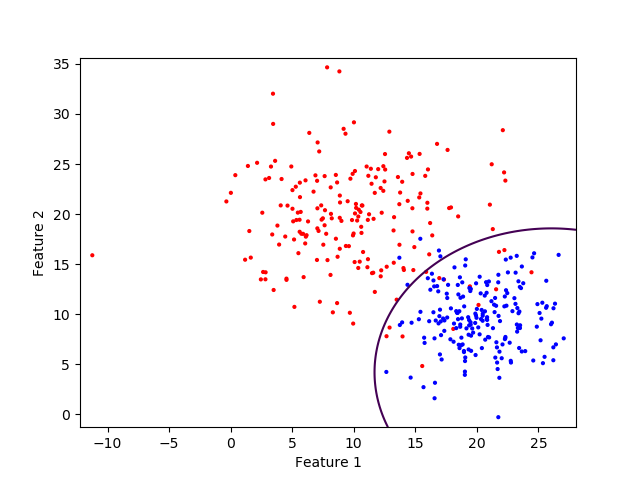
\includegraphics[width=\textwidth]{Part1_Task1.png} % first figure itself
            \caption*{Task 1: Different Covariances}
        \end{minipage}\hfill
        \begin{minipage}{0.5\textwidth}
            \centering
            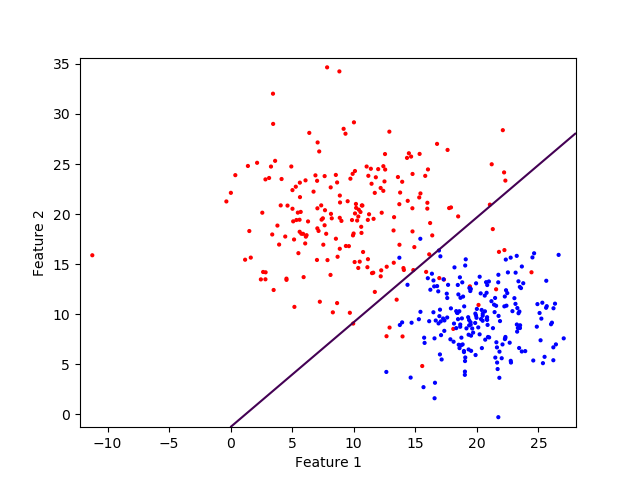
\includegraphics[width=\textwidth]{Part1_Task2.png} % second figure itself
            \caption*{Task 2: Same Covariance}
        \end{minipage}
        \caption{The plots for \texttt{binclass.txt}}
    \end{figure}
    \begin{figure}[h]
        \centering
        \begin{minipage}{0.5\textwidth}
            \centering
            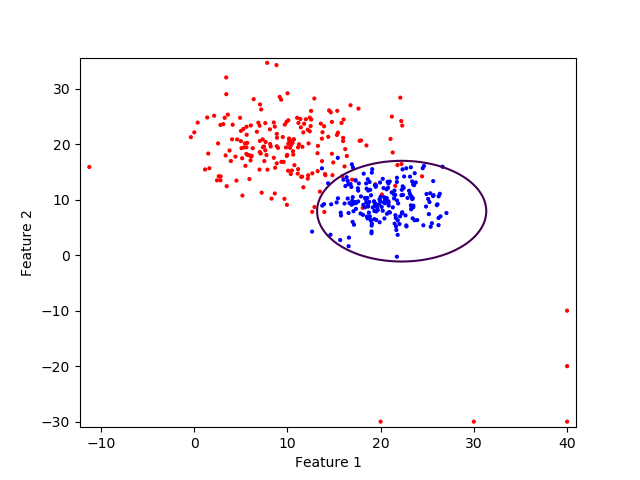
\includegraphics[width=\textwidth]{Part2_Task1.png} % first figure itself
            \caption*{Task 1: Different Covariances}
        \end{minipage}\hfill
        \begin{minipage}{0.5\textwidth}
            \centering
            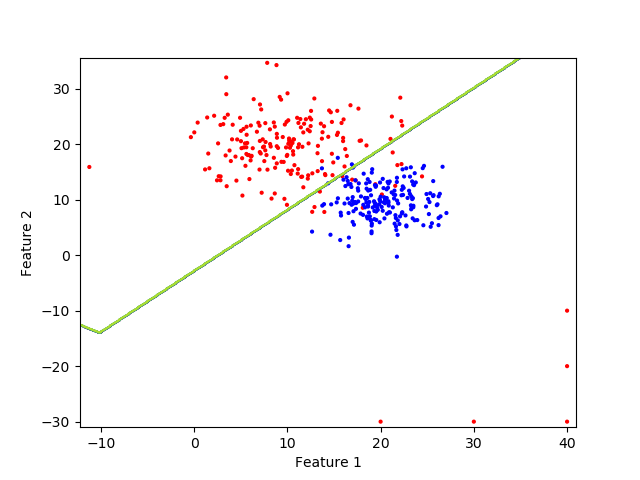
\includegraphics[width=\textwidth]{Part2_Task2.png} % second figure itself
            \caption*{Task 2: Same Covariance}
        \end{minipage}
        \caption{The plots for \texttt{binclassv2.txt}}
    \end{figure}

    For both the datasets \texttt{binclass.txt} as well as \texttt{binclassv2.txt}, having separate covariance matrices for the 2 classes does a better job of classifying the points.
    In general cases too, we expect having different covariance for each of the classes will do better. Having same covariance matrix for 2 classes means that the model produces a Linear Decision Boundary between them.

    \begin{figure}[h]
        \centering
        \begin{minipage}{0.5\textwidth}
            \centering
            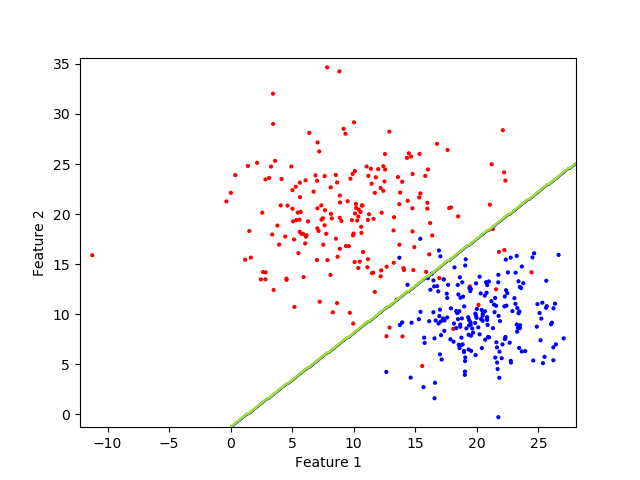
\includegraphics[width=\textwidth]{Part1_Task3.png} % first figure itself
            \caption*{Linear Kernel SVM for \texttt{binclass.txt}}
        \end{minipage}\hfill
        \begin{minipage}{0.5\textwidth}
            \centering
            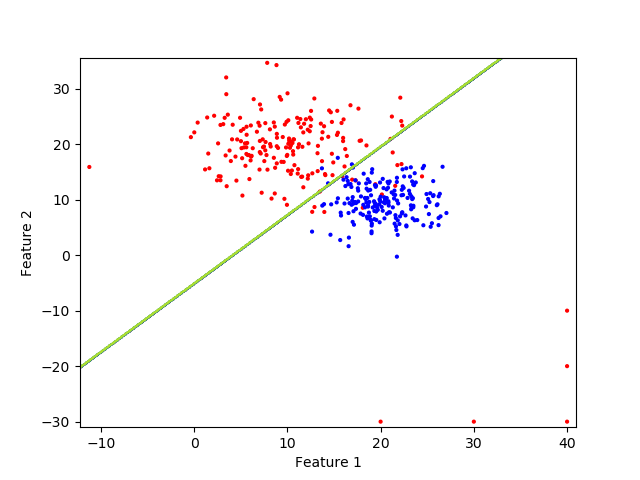
\includegraphics[width=\textwidth]{Part2_Task3.png} % second figure itself
            \caption*{Linear Kernel SVM for \texttt{binclassv2.txt}}
        \end{minipage}
        \caption{SVM Plots generated using \textsl{scikit-learn} library.}
    \end{figure}

\end{mlsolution}


\end{document}
